% ============================ Enrico Ribiani 16-03-2021 ====================================================================
% Base per i documenti  
\documentclass[12pt]{article}
% ------------ pacchetti necessari ----------------
\usepackage[a4paper, total={6in, 8in},margin=1in]{geometry} % formattazione decente della pagina
\usepackage{graphicx}                            % need for figure
\usepackage{amsmath}
\usepackage{amsfonts}                            % if you want the fonts
\usepackage{amssymb}                             % if you want extra symbols
\usepackage{graphicx}  
\renewcommand{\figurename}{Figura}  
\renewcommand{\contentsname}{Indice}                        % need for figures
\usepackage{mathptmx}
\usepackage{float}                               % serve per mettere tabelle e immagini dove si vuole 
\usepackage[utf8]{inputenc}
\usepackage{textcomp}
\usepackage[hang,flushmargin,bottom]{footmisc}   % footnote format
\usepackage{fancyhdr, lastpage}
\usepackage{titlesec}
\usepackage[table,dvipsnames]{xcolor}
%\pagestyle{fancy}
%\renewcommand{\headrulewidth}{0pt}
%\renewcommand*\contentsname{Indice}
\titleformat{\section}{\normalsize\bfseries}{\thesection.}{1em}{}	% required for heading numbering style
\titleformat*{\section}{\Large\bfseries}
\titleformat*{\subsection}{\large\bfseries}
%\usepackage{siunitx}
%\usepackage{tikz}
\usepackage{circuitikz}
%\usepackage[siunitx]{circuitikz}
\usepackage{multirow}
\usepackage{tikz}
\usepackage{amsmath}
\usetikzlibrary{angles,quotes}
\usepackage{placeins}
%===================links=================
\usepackage{hyperref}
\hypersetup{
    colorlinks=true,
    linkcolor=Sepia,
    filecolor=Green,      
    urlcolor=Cyan,
    pdftitle={SAMPLE},
    pdfpagemode=FullScreen,
    }
%===================inizio pagina del titolo=================
\begin{document}
    \begin{titlepage}
    \begin{center}
% ------------------ inizio immagine logo ----------
\begin{figure}
    \centering
    \includegraphics{~/varie/logo.png}
    \label{fig:logo}
\end{figure}
% ------------------ fine immagine logo ----------
% ------------------ fine immagine logo ----------
-------------------------------------------------------------------------------------\\
\vspace{2\baselineskip}
\large Enrico Ribiani\\
\large 4AUB\\
\vfill

\Huge{\textbf{Esperienza laboratoriale bipolo ohmico-capacitivo}}\\
\vfill

\LARGE{esperienza n°1}\\
\vfill
\large{01-10-2021}
\end{center}
%=============== fine pagina titolo ===============
\end{titlepage}
\tableofcontents
\vskip 1cm
\section{Scopo:Verificare il comportamento di un bipolo ohmico-capacitivo sperimentalmente.}
    \subsection{Materiale}
    \begin{itemize}
        \item Breadboard
        \item Condensatore da \textit{10nF}
        \item Resistenza da \textit{10k$\Omega$}
    \end{itemize}
    \subsection{Strumenti}
    \begin{itemize}
        \item Generatore di funzione
        \item Oscilloscopio
    \end{itemize}
        \subsubsection{Schema}
        \begin{circuitikz}[american voltages]
            \draw
                (0,0) -- (0,-0.2) node[ground]{}    
                to[vsourcesin, l_=\textit{v(t)}] (0,4)
                (0,4) to [short, *-, l=Ch1] (0,4)
                to[american resistor,  l_=R \textit{10k$\Omega$}, i=\textit{i(t)}] (4,4) -- (4,0)
                (4,4) to [short, *-, l=Ch2] (4,0) %label ch2 da fixare
                to[capacitor, l=C\textit{10nF}] (0,0)
                (0,0) to [short, *-] (0,0)
            ;
        \end{circuitikz}

        \vskip 1cm
        
        \begin{center}
            Il primo circuito verrà utilizzato per effettuare le misure su R mentre il secondo che è l'euqivalente del primo solo con R e C invertite per effettuare
            le misurazioni sul conduttore. 
        \end{center}
       
        \vskip 1cm

   \begin{circuitikz}[american voltages]
    \draw
        (0,0) -- (0,-0.2) node[ground]{}    
        to[vsourcesin, l_=\textit{v(t)}] (0,4)
        (0,4) to [short, *-, l=Ch1] (0,4)
        to[capacitor, l=C \textit{10nF}] (4,4) -- (4,0)
        (4,4) to [short, *-, l_=Ch2,i=\textit{i(t)}] (4,0) %label ch2 da fixare
        to[american resistor,  l_=R \textit{10k$\Omega$}] (0,0)
        (0,0) to [short, *-] (0,0)
    ;
\end{circuitikz}

\section{Cenni teorici}
    \subsection{Generalità bipolo RC}
    Il bipolo ohmico-capacitivo è formato da una sorgente di alimentazione, un resistore (R) e un condensatore (C) con resistenza e 
    capacità costante, mentre la tensione di alimentazione varia in modo sinusoidale. Questo circuito può esere in serie o in parallelo,
    in questa esperienza laboratoriale prendiamo in considerazione quello in serie.\\
    Nel bipolo sono presenti 3 tensioni, la tensione ai capi del resistore $\vec{V_R}$ quella ai capi del condensatore $\vec{V_C}$ e quella totale $\vec{V}$, 
    mentre consideriamo solamente la corrente totale $\vec{I}$ .\\
    Come nel caso dei bipoli puramente resistivi $\vec{V_R}$ sarà in fase con la corrente, analogamente come nel bipolo puramente capacitivo $\vec{V_C}$ sarà sfasato 
    di 90° o ($\frac{\pi}{2}$) in ritardo rispetto alla corrente.\\
    In base alla frequenza e alla capacità del condensatore la tensione \textit{V} sarà più o meno sfasata.
    \subsection{Previsione comportamento}
    Una volta collegato il circuito all'oscilloscopio e regolato il generatore di funzione con i parametri desiderati ci aspetteremo di vedere due onde sinusoidali
    una sfasata all'altra di un tempo \textit{t} in ritardo, quella in ritardo deve essere quella ai capi del condensatore.\\
\section{Procedimento/Analisi}
    Dopo aver ricevuto il materiale si procede a montare il circuito sulla breadboard secondo il primo schema, dopodichè si procede a collegare l'oscilloscopio.\\
    Prima di collegare il generatore di funzione si setta l'onda sinusoidale a una $V_{PP}$ di 7V con una frequenza di $1Hz$.\\
    Dopo aver settato il generatore di funzione si collega al circuito, si controlla di aver collegato tutto correttamente e si preme sul pulsante output che 
    fa partire l'onda.\\
    Si procede settanddo l'oscilloscopio in modo da poter vedere in modo chiaro entrambe le onde, prefiribilmente con la stessa scala, il passo seguente 
    è prendere le misure della  $V_{PP}$ su C e del ritardo ($t$) di un'onda sull'altra.\\
    Segnato i valori misurati sulla tabella si procede a invertire il condensatore e il resistore per effettuare le stesse misurazioni su R.\\
    Con i valori delle tabelle si vanno ad effettuare i calcoli per calcolare le incognite, si calcolano le tensioni efficaci ai capi della resistenza e del condensatore
    per poi calcolare la reattanza capacitiva, lo sfasamento, la corrente e l'induttanza.\\ 
    \subsection{Foto}
    \begin{figure}[!h]
        \centering
        \includegraphics[scale=0.2]{images/photo_2021-10-06_16-31-10.jpg}
        \caption{$V_R$ Ch1 (giallo)}
    \end{figure}
    
   
    \begin{figure}[!h]
        \centering
        \includegraphics[scale=0.2]{images/photo_2021-10-06_16-30-22.jpg}
        \caption{$V_C$ Ch2 (blu)}
    \end{figure}
    \FloatBarrier
\subsection{Tabelle}    
\vspace{1cm}        
\begin{table}[!h]
            \centering
            
        \begin{tabular}{|p{2cm}|p{2cm}|p{2cm}|}
        \hline
        \rowcolor{BurntOrange} \multicolumn{3}{|c|}{C} \\
        \hline\hline
        \rowcolor{Apricot} Vpp & t$\pm$ & $\varphi$  \\ 
         \hline
        \rowcolor{Peach}6V & -90$\mu$s & -32,4°  \\
         
         \hline
        \end{tabular}
            \vspace{1cm}
        \begin{tabular}{|p{2cm}|p{2cm}|p{2cm}|} 
            \hline
            \rowcolor{BurntOrange} \multicolumn{3}{|c|}{R} \\
            \hline\hline
            \rowcolor{Apricot} Vpp & t$\pm$ & $\varphi$  \\ 
             \hline
            \rowcolor{Peach}3,56V & 170$\mu$s & 61,2°  \\
             
             \hline
            \end{tabular}
    \end{table}
   
    \subsection{Calcoli}
    Incognite: $\vec{Z}$, $V$, $V_R$, $V_C$, $I$.\\
    \\
    $Vp=\frac{Vpp}{2}=\frac{7V}{2}=3,5V$\\
    $V=\frac{Vp}{\sqrt{2}}=\frac{3,50V}{\sqrt{2}}=2,47V$\\
    \\
    $Vp_R=\frac{Vpp_R}{2}=\frac{3,56V}{2}=1,78V$\\
    $V_R=\frac{Vp_R}{\sqrt{2}}=\frac{1,78V}{\sqrt{2}}=1,26V$\\
    \\
    $Vp_C=\frac{Vpp_C}{2}=\frac{6V}{2}=3V$\\
    $V_C=\frac{Vp_C}{\sqrt{2}}=\frac{3V}{\sqrt{2}}=2,12V$\\
    \\
    $X_c=\frac{1}{\omega C}=\frac{1}{2\pi f C}=\frac{1}{2\pi\cdot 1000 \cdot 10^{-9}}=15,915k\Omega$\\
    \\
    $\varphi_C:2\pi=t:T$ \\
    $\varphi_C=\frac{2\pi \cdot t}{T}$\\
    $\varphi_C=\frac{360 \cdot (-90\cdot 10^{-6})}{0,001}=-32,4$°\\
    \\
    $\varphi_R:2\pi=t:T$ \\
    $\varphi_R=\frac{2\pi \cdot t}{T}$\\
    $\varphi_R=\frac{360 \cdot (170\cdot 10^{-6})}{0,001}=61.2$°\\
    \\
    $\varphi=arctg(\frac{-X_C}{R})=arctg(\frac{15,9}{10}k\Omega)=-57.8$°\\
    \\
    $\vec{Z}=(R-jX_C)=(10-15,915)k\Omega$\\
    \\
    $Z=\sqrt{10000^2+15,9^2}=18,8k\Omega$\\
    \\
    $I=\frac{V}{Z}=\frac{2,47V}{18,8k\Omega}=13 mA$\\
\section{Conclusioni}
L'esperienza ha verificato correttamente il comportamento di un bipolo ohmico-capacitivo soddisfacendo lo scopo.\\
Abbiamo osservato che gli sfasamenti sono corretti, $V_C$ è in ritardo rispetto alla corrente mentre $V_R$ ha uno sfasamento nullo, ossia è in fase
la tensione totale appunto risulta avere uno sfasamento $\varphi$ negativo. Lo sfasamento totale tra tensione e corrente è di 90°.\\
L' angolo $\varphi$ non risulta rappresentato dal diagramma vettoriale perché il metodo di calcolo utilizzato considera $I$ sull'asse delle ascisse mentre i nostri valori
avevano uno sfasamento iniziale non nullo.
\subsection{Diagramma vettoriale}
\textit{u=1V}\\
%\begin{tikzpicture}
 % \draw[thin,gray!40] (-4,-6) grid (6,4);
  %\draw[->] (-3,0)--(5,0) node[right]{$x$};
  %\draw[->] (0,-5)--(0,3) node[above]{$y$};
  %\draw[line width=2pt,orange,-stealth](0,0)--(4,0) node[anchor=south west]{$\boldsymbol{\vec{I}}$};
  %\draw[line width=2pt,green,-stealth](0,0)--(2.48,0) node[anchor=south west]{$\boldsymbol{\vec{V_R}}$};
  %\draw[line width=2pt,blue,-stealth](0,0)--(0,-4.24) node[anchor=north east]{$\boldsymbol{\vec{V_C}}$};
  %\draw[line width=2pt,purple,-stealth](0,0)--(2.48,-4.24) node[anchor=north east]{$\boldsymbol{\vec{V}}$};
  
   
  %angolo

%\draw [fill=green!30] (a) -- ++(1cm,0) arc(0:{atan(1/2)}:1cm) node[midway,right] {$\alpha$} -- cycle;
%\coordinate (a) at (0,0);
%\coordinate (b) at (2.48,0);
%\coordinate (c) at (2.48,-4.24);

%\draw pic[draw,fill=green!30,angle radius=1cm,"$\varphi$-57.8°" shift={(15mm,-2mm)}] {angle=c--a--b};
%\end{tikzpicture}

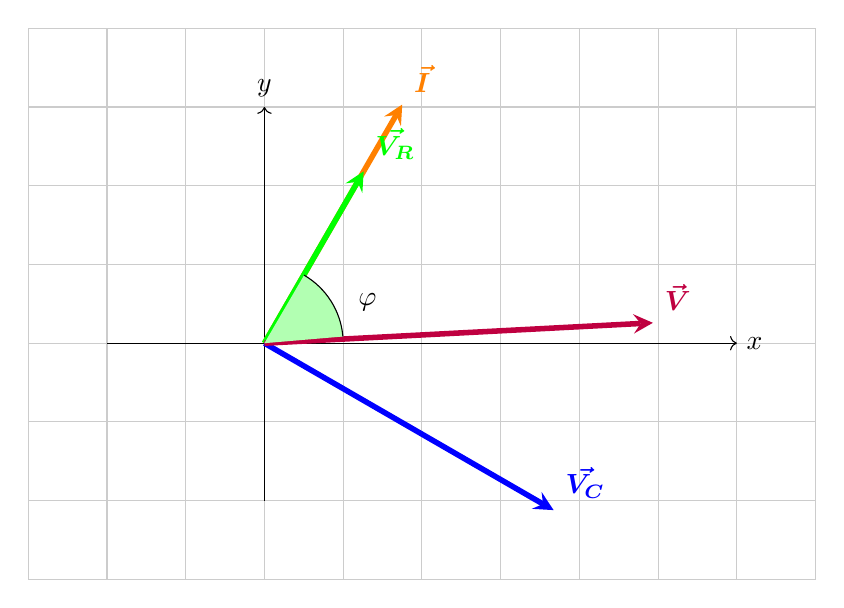
\begin{tikzpicture}
    \draw[thin,gray!40] (-3,-3) grid (7,4);
    \draw[->] (-2,0)--(6,0) node[right]{$x$};
    \draw[->] (0,-2)--(0,3) node[above]{$y$};
    \draw[line width=2pt,orange,-stealth] (0,0) -- (60:3.5cm) node[anchor=south west]{$\boldsymbol{\vec{I}}$};
    \draw[line width=2pt,green,-stealth] (0,0) -- (60:2.52cm) node[anchor=south west]{$\boldsymbol{\vec{V_R}}$};
    \draw[line width=2pt,blue,-stealth] (0,0) -- (-30:4.24cm) node[anchor=south west]{$\boldsymbol{\vec{V_C}}$};
    \draw[line width=2pt,purple,-stealth] (0,0) -- (3:4.94cm) node[anchor=south west]{$\boldsymbol{\vec{V}}$};
    
    %angolo
  
  %\draw [fill=green!30] (a) -- ++(1cm,0) arc(0:{atan(1/2)}:1cm) node[midway,right] {$\alpha$} -- cycle;
  \coordinate (a) at (0,0);
  \coordinate (c) at (2,0.17);
  \coordinate (b) at (3.5,6);
  
  \draw pic[draw,fill=green!30,angle radius=1cm,"$\varphi$" shift={(8mm,2mm)}] {angle=c--a--b};
  \end{tikzpicture}

\end{document}
